 \documentclass[ngerman]{scrartcl} %lädt die Dokumentklasse
                                %Artikel von Koma-Skript, als Option
                                %übergebe ich, dass ich die Trennung
                                %nach neuer deutscher Rechtschreibung
                                %wünsche
\usepackage[utf8]{inputenc}
 \usepackage[ngerman]{babel}
\usepackage{color}
\usepackage[T1]{fontenc}
\usepackage[pdfborder={0 0 0}]{hyperref}
\usepackage[a4paper,lmargin={4cm},rmargin={2cm},
tmargin={2.5cm},bmargin = {2.5cm}]{geometry}
\usepackage{amssymb}
\usepackage{graphicx}
\usepackage{amsthm}
\usepackage{graphicx}
\usepackage{url} 

 \begin{document}
\tableofcontents
\newpage
 
\section{Einleitung}        
\label{sec:Einleitung-1}       
Aufgrund der technologischen Entwicklung in den letzten Jahren sind immer kleinere Geräte möglich, die immer mehr Funktionen übernehmen können. Diese Geräte werden in immer mehr Bereichen des täglichen Lebens eingesetzt und ermöglichen so neue Anwendungsgebiete, die sich nicht mehr nur auf den heimischen Computer beschränken. Eine dieser Entwicklungen ist der sogenannte ``Amazon Dash Button'', der von Amazon im Jahr 2015 veröffentlicht und auf den Markt gebracht wurde. 
Dieser kleine Button wurde entwickelt, um den Bestellprozess beim Internethändler zu vereinfachen. Über eine WLAN Verbindung und eine einmalige kurze Konfiguration wird der Kaufprozess für ein zuvor definiertes Produkt angestoßen. Dazu muss nur der Button betätigt werden und die Bestellung wird aufgegeben. (vgl. \cite{Amazon.})

Im Rahmen dieser Studienarbeit werden diese Prozesse untersucht und eine offenere Lösung entwickelt. Bei der ersten Betrachtung des Produkts fällt nämlich auf, dass es für den Kunden einige Nachteile gibt. Zum einen ist er an den Internethändler Amazon gebunden, da dieser nur die Bestellung über sein Angebot ermöglicht. Weiterhin ist es nicht möglich bei der Betätigung des Buttons den aktuellen Preis des Produkts zu sehen. Das bedeutet, dass der Kunde das übliche Produkt bestellt und den genauen Preis nicht weiß. Diese zwei Nachteile sollen durch eine offene und durch den Nutzer konfigurierbare Lösung behoben werden. Auf den folgenden Seiten wird auf die Theorie und die Entwicklung der Lösung detailliert eingegangen und zudem der Amazon Dash Button genauer untersucht.

\newpage
\section{Überblick der vorgestellten Lösung}
\label{sec:Überblick der vorgestellten Lösung-1}
Die vorgestellte Lösung soll auf freie Technologien zurückgreifen und somit für den Nutzer nachvollziehbar sein. Das erklärte Ziel ist es, über Buttons einen Einkaufszettel zusammenzustellen, der dem Nutzer dann zur Verfügung gestellt wird. Dazu wird mit sogenannten Mikrocontrollern und Einplatinencomputern die benötigte Infrastruktur realisiert und aufgebaut. Damit die Daten nicht außerhalb der Kontrolle des Nutzers liegen, wird ein zentraler Server im Netzwerk benötigt. Dieser zentrale Server empfängt zudem die entsprechenden Signale der Clients, die in diesem Falle die Buttons sind. 

\newpage

\section{Theorie}        
\label{sec:Theorie-1}  

\subsection{UDP}
\label{sec:UDP-1}
UDP steht für ``User-Datagram-Protocol'' und ist ein verbindungsloses Transportprotokoll. Im OSI-7-Schichten Modell arbeitet es auf der Transportebene und ist für die Zustellung von Netzwerkpaketen von einem Sender zu einem Empfänger zuständig. Im Vergleich zum Transportprotokoll TCP, welches verbindungsorientiert arbeitet, ist es wesentlich einfacher zu verarbeiten, da beispielsweise der Header wesentlich kleiner ist. Allgemein ist es sehr minimal gehalten und dadurch sehr einfach zu implementieren und für sehr einfache Anwendungszwecke geeignet. Allerdings ist auch zu erwähnen, dass es keine Empfangsbestätigung gibt und die Daten nach dem Absenden nicht weiter kontrolliert werden. Somit können die Daten auch im Netzwerk verloren gehen und der Nutzer bemerkt es nicht. \\

Der einfache Header des UDP Protokolls besteht nur aus vier Attributen. Diese jeweils 16 Bit großen Felder enthalten den Quellport, den Zielport, die Checksumme zur Überprüfung des Inhalts und die Länge des gesamten Pakets. Insgesamt ist der Header somit 8 Byte groß und im Vergleich zu TCP mindestens um den Faktor 1.5 kleiner als ein TCP Header. TCP nutzt einen Header der aus elf Feldern besteht die insgesamt mindestens 20 Byte Platz benötigen. Da der Header jedoch um einige Felder erweitert werden kann, ist es möglich, dass er noch mehr Platz benötigt. (vgl. \cite{ElektronikKompendium.}\cite{.}\cite{.23.02.2016})
 
\subsection{Webserver: Nginx}
\label{sec:Webserver: Nginx-1} 
 
\subsection{Arduino}
\label{sec:Arduino-1} 

\subsection{WLAN-Chipsatz}
\label{sec:WLAN-CHipsatz-1} 
 
\subsection{REST}        
\label{sec:REST-1}  

\cite{Tilkov.2015}
 
 
\newpage
 
\section{Auswahl der Hardware}        
\label{sec:Auswahl der Hardware-1}  

In den folgenden Kapiteln wird die ausgewählte Hardware des Projektes vorgestellt. Dabei wird zuerst auf die technischen Merkmale eingegangen und dann auf den genauen Verwendungszweck im Projekt. 

\subsection{Raspberry PI}        
\label{sec:Raspberry PI-1} 

\subsubsection{Vorstellung des Raspberry PI}        
\label{sec:Vorstellung des Raspberry PI-1} 

Das Raspberry PI ist ein Einplatinencomputer, den es in verschiedenen Ausführungen gibt. Je nach Ausführung variieren die Ausstattungsmerkmale. Zu den Grundsätzlichen Ausstattungsmerkmalen gehören eine CPU, unterschiedlich viel RAM und eine iGPU Einheit. Er wurde von der Raspberry PI Foundation entwickelt und hatte das ursprüngliche Ziel einen günstigen Computer für den Schulunterricht bereitzustellen. Daher ist es auch möglich eine vollständige Linux Distribution als Betriebssystem zu nutzen und es wurde sogar eine speziell angepasste Distribution veröffentlicht, die Raspbian bezeichnet wird. 
Aufgrund der verschiedenen Möglichkeiten wird er aber mittlerweile auch in vielen anderen Anwendungsgebieten genutzt. Insbesondere die neueren Modelle, die mit mehreren USB Ports, GPIO Pins, einem Ethernet Port und weiteren Anschlüssen ausgestattet sind, werden auch in verschiedensten Projekten privater Personen genutzt. Ein weiteres Merkmal ist die Größe des Raspberry PI's, die mit maximal 93mmx63.5mmx20mm sehr klein ausfällt. Zusätzlich gibt es diverses, bereits für den Raspberry PI ausgelegtes, Zubehör, welches weitere Erweiterungsmöglichkeiten bietet. So gibt es Kameras, Gehäuse, kleine Displays und WLAN Sticks, die den Funktionsumfang erweitern. So wurden bereits diverse Projekte vorgestellt, die zeigen, dass die Einsatzmöglichkeiten des Raspberry Pis wesentlich größer sind. (vgl. \cite{.28.12.2016} \cite{.28.01.2017})
\\
\begin{figure}[!htb]
	\centering
	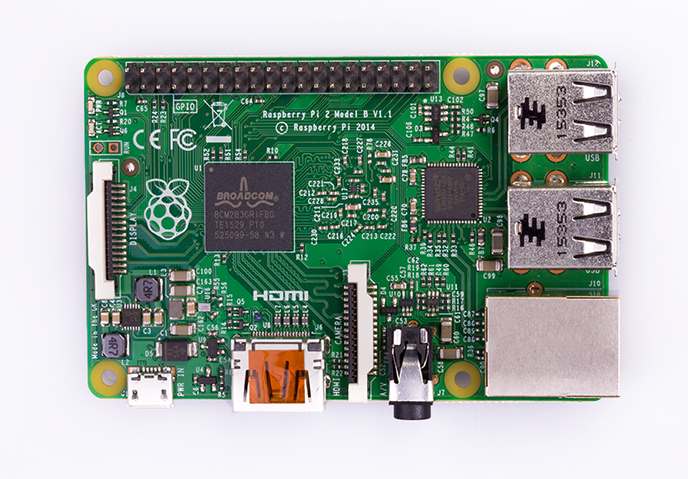
\includegraphics[scale=0.5]{Raspberry-Pi-2-web.png}
	\caption[RaspberryPi Modell 2 B]{RaspberryPi Modell 2 B+,\\ Quelle: https://www.raspberrypi.org/wp-content/uploads/2016/02/Raspberry-Pi-2-web.jpg}
\end{figure}


\subsubsection{Verwendung im Projekt}        
\label{sec:Verwendung des Raspberry PI-1} 
Der Raspberry PI wird für das Projekt genutzt, um einen zentralen Server bereitzustellen. Aufgrund der technischen Merkmale kann zeitgleich ein Webserver und ein Datenbankserver betrieben werden. Zudem kann über die USB Anschlüsse ein WLAN Stick angeschlossen werden, sodass die Buttons über das WLAN Netzwerk des Raspberry PIs zum zentralen Server kommunizieren können. Dazu muss mithilfe eines Skriptes der WLAN Stick von einem Empfänger zu einem Sender bzw. Access Point umfunktioniert werden. Um die dann eingehenden Nachrichten der Buttons empfangen zu können, muss zudem noch ein entsprechendes Skript im Hintergrund laufen, dass die Daten empfängt. Aufgrund von vier parallel laufenden Prozessen (Webserver, Datenbankserver, WLAN Skript und Skript zum Empfangen der Daten) wird einiges an Rechenleistung benötigt, die der Raspberry Pi allerdings aufbringen kann. 
Der Webserver auf dem Raspberry Pi wird dabei sowohl für das Frontend als auch für das Backend benötigt werden. Das Frontend soll dem Nutzer die Möglichkeit geben, die Liste von Waren zu verwalten und die Buttons zu konfigurieren bzw. Hilfestellung zur Einrichtung zu geben. Das Backend des Servers wird unter anderem aus einer REST API bestehen, die sowohl die Anfragen des Webservers verarbeitet als auch die Anfragen an die Datenbank im allgemeinen. 
Der Datenbankserver im Hintergrund wird die benötigte Datenbank entsprechend verwalten. 

\subsection{``Pretzelboard''}        
\label{sec:''Pretzelboard''-1} 

\subsubsection{Vorstellung des ``Pretzelboard''}        
\label{sec:Vorstellung des ``Pretzelboard''} 
Das ``Pretzelboard'' ist ein sogenanntes Elektronikmodul, dass unter verschiedenen Namen bekannt ist. Neben ``Pretzelboard'' ist der Name ``NanoESP-Board'' ebenfalls bekannt. Die Besonderheit des Boards ist ein bereits angeschlossenes WLAN Modul, welches sowohl als Sender als auch Empfänger arbeiten kann. Da es zudem den gleichen Microcontroller wie das bekanntere Microcontrollerboard ``Arduino Uno'' nutzt, kann die Entwicklungsumgebung von Arduino zur Entwicklung von Software genutzt werden. 
Der Vorteil der bereits erfolgten Kombination und Verdrahtung von WLAN Modul und Microcontroller liegt darin, dass der Nutzer dies nicht mehr machen muss und somit wesentlich weniger Kenntnisse vorausgesetzt werden müssen. (vgl. \cite{.b}\cite{.kafka}\cite{FranzisVerlagGmbH.27.11.2015})


\subsubsection{Verwendung im Projekt}        
\label{sec:Verwendung des ``Pretzelboard''} 
Das ``Pretzelboard'' wird im Projekt als Button genutzt. Sowohl die kleine Größe als auch die bereits vorhandene WLAN Funktionalität sorgen dafür, dass sich das Board dafür besonders gut eignet. Aufgrund der Tatsache, dass es sich bezüglich der Programmierung nicht von einem Arduino Board unterscheidet, besteht die Möglichkeit, dass auf das Wissen und den Support einer bereits größeren Community zurückgegriffen werden kann. 
Da sich das Board zudem auf ein Elektroniksteckboard setzen lassen kann, ist auch die Verbindung mit einem Button und Statusleuchten möglich. Nach der erfolgreichen Montage kann dann das entsprechende Programm aufgespielt werden und bei vorhandener Stromversorgung kann die entsprechende Nachricht über das WLAN Netzwerk an den Empfänger gesendet werden. 

\newpage

\section{Umsetzung des Projektes}        
\label{sec:Umsetzung des Projektes-1}  

\subsection{Architektur und Zusammenspiel der Komponenten}        
\label{sec:Architektur und Zusammenspiel der Komponenten-1} 

Einbindung von \nameref{sec:Auswahl der Hardware-1}

\subsection{Einrichtung der Hardware}  
\label{sec:Einrichtung der Hardware-1} 

\subsubsection{Einrichtung des Raspberrys}  
\label{sec:Einrichtung des Raspberrys-1}

\paragraph{Einrichtung des WLAN Access Points}  
\label{sec:Einrichtung des WLAN Access Points-1} 

\paragraph{Einrichtung des UDP Empfängers}  
\label{sec:Einrichtung des UDP Empfängers-1} 

\subsubsection{Einrichtung des ``Pretzelboards''}  
\label{sec:Einrichtung des ``Pretzelboards''-1}

\subsection{Entwicklung der Webanwendung}  
\label{sec:Entwicklung der Webanwendung-1} 

\subsubsection{Aufbau und Entwicklung der REST API}  
\label{sec:Aufbau und Entwicklung der REST API-1}

\subsubsection{Aufbau und Entwicklung des Frontends}  
\label{sec:Aufbau und Entwicklung des Frontends-1}

\subsection{Entwicklung und Einrichtung der Datenbank}  
\label{sec:Entwicklung und Einrichtung der Datenbank-1} 

\newpage

\section{Ergebnis des Projektes}        
\label{sec:Ergebnis des Projektes-1}  

\newpage

\section{Fazit und Ausblick}        
\label{sec:Fazit und Ausblick-1}  

\newpage


\addcontentsline{toc}{section}{Literaturverzeichnis}
\bibliographystyle{unsrt}  
\bibliography{Literatur}

\newpage

\addcontentsline{toc}{section}{Abbildungsverzeichnis}

\listoffigures

 \end{document}